\PassOptionsToPackage{table}{xcolor}
\documentclass[aspectratio=169, 11pt]{beamer}

% ============================================
% THEME
% ============================================
\usetheme{metropolis}
\usecolortheme{default}

\definecolor{darkblue}{RGB}{0, 51, 102}
\definecolor{darkred}{RGB}{139, 0, 0}
\definecolor{darkgreen}{RGB}{0, 100, 0}

\setbeamercolor{frametitle}{bg=darkblue, fg=white}
\setbeamercolor{title}{fg=darkblue}
\setbeamercolor{structure}{fg=darkblue}
\setbeamertemplate{navigation symbols}{}
\setbeamertemplate{footline}[frame number]

% ============================================
% PACKAGES
% ============================================
\usepackage{graphicx}
\usepackage{booktabs}
\usepackage{amsmath}
\graphicspath{{figures/}{../final report/figures/}}

% ============================================
% TITLE
% ============================================
\title{When Regional Favoritism Fades}
\subtitle{Nightlights and Pollution in Leader Birth Regions}
\author{Richard Schulz \and Muhammad Majid Altaf \and Ruby Wang}
\institute{INFO 288: Big Data and Development \\ Prof.\ Joshua Blumenstock}
\date{Spring 2026}

\begin{document}

% --- Title ---
\begin{frame}[plain]
    \titlepage
\end{frame}

% --- Visual hook ---
{
\setbeamercolor{background canvas}{bg=black}
\setbeamercolor{normal text}{fg=white}
\setbeamercolor{alerted text}{fg=white}
\setbeamercolor{frametitle}{bg=black, fg=white}
\begin{frame}{Hambantota, Sri Lanka at night}
    \centering
    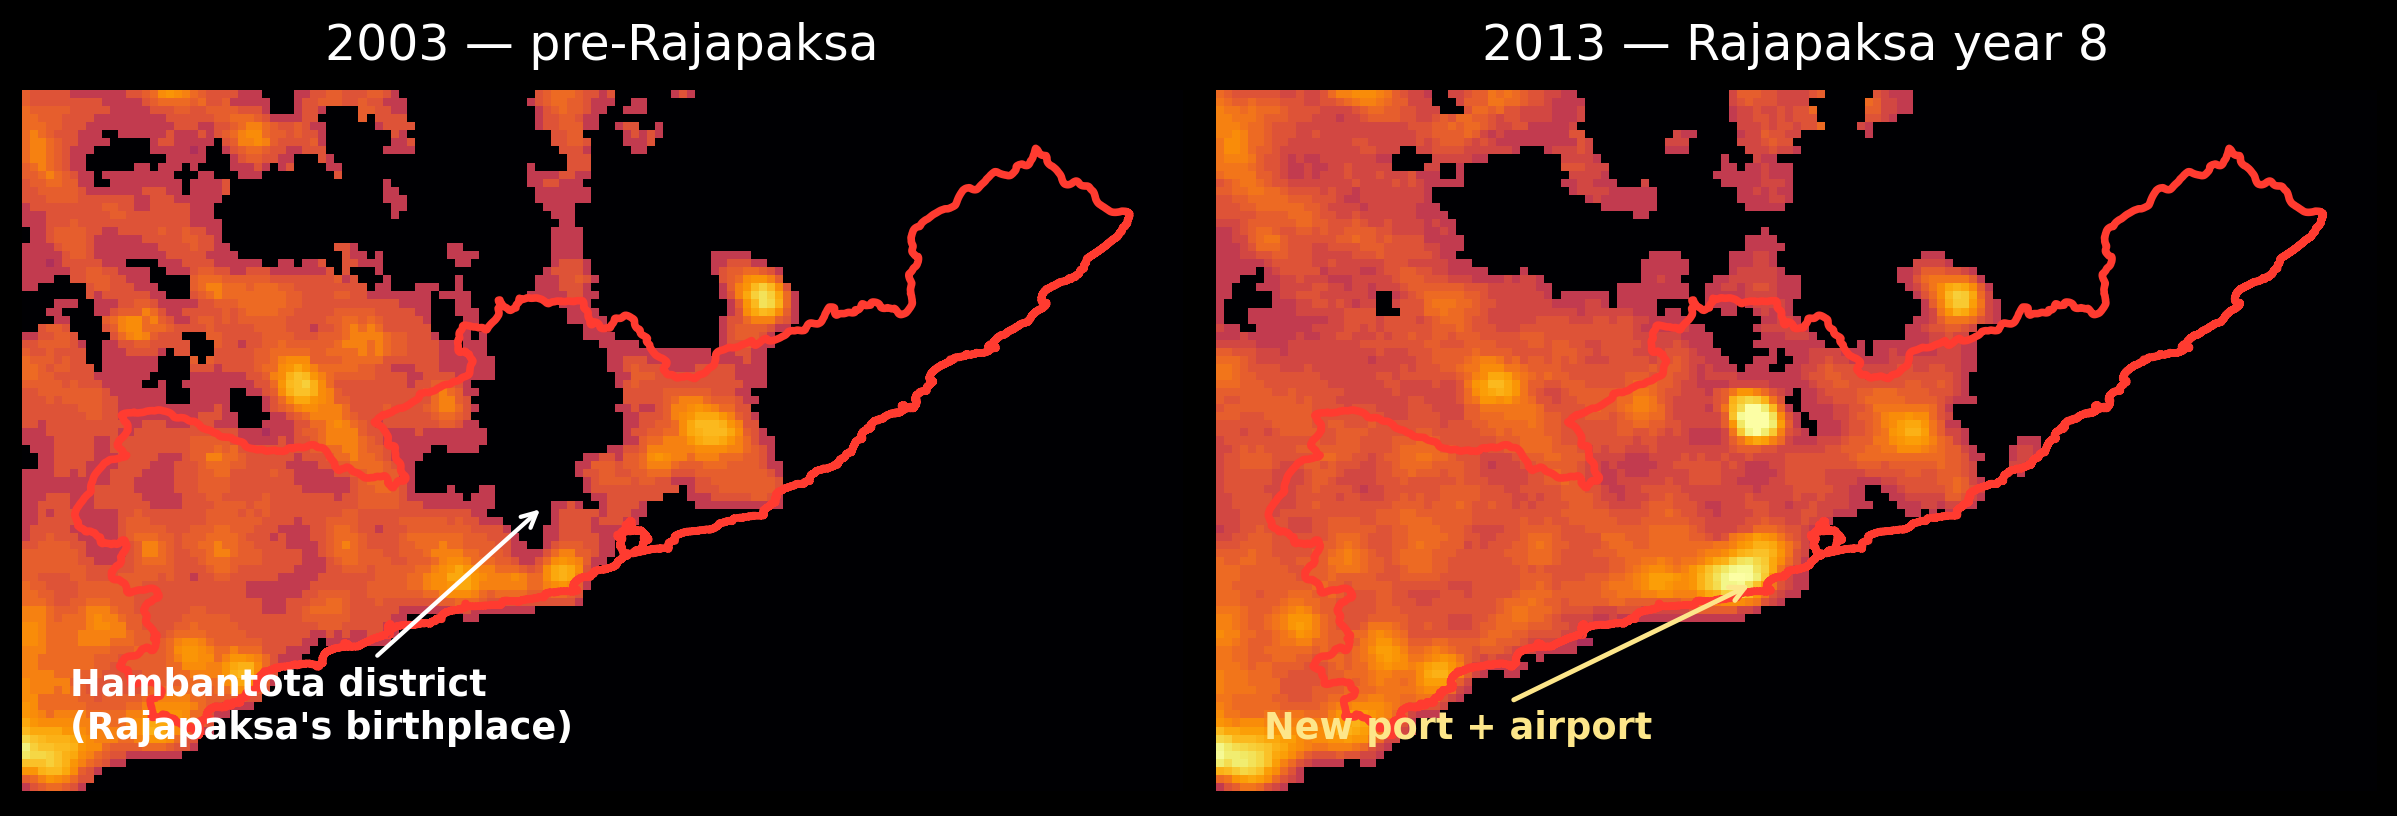
\includegraphics[width=0.92\linewidth]{hambantota_nightlights.png}

    \vspace{0.4em}
    {\color{white}\footnotesize Rajapaksa took office in 2005. By 2013, his home district had a \$1.5B Chinese-financed port, an international airport named after him, a cricket stadium, and a conference center. Most are barely used.}
\end{frame}
}

% --- The pattern ---
\begin{frame}{The pattern}
    \begin{itemize}
        \item Leaders direct resources to where they're \textbf{from}
        \item Hodler \& Raschky (\textit{QJE}, 2014) show this globally in satellite nightlights
        \item The effect is largest in Sub-Saharan Africa
    \end{itemize}

    \vspace{1em}
    \begin{block}{Our question}
        Does it \textbf{still hold} after 2005?
    \end{block}
\end{frame}

% --- This project ---
\begin{frame}{This project}
    \textbf{Two questions:}
    \begin{enumerate}
        \item Does the birth-region nightlights effect \textbf{replicate after 2005}?
        \item If not, did favoritism shift from \emph{more} growth to \emph{cleaner} growth? (``green favoritism'')
    \end{enumerate}

    \vspace{1em}
    \textbf{Preview:}
    \begin{itemize}
        \item Long DMSP (1992--2013): replicates ($\beta = 0.013$, $p = 0.030$)
        \item Post-2005: estimates collapse, and no subsample brings them back
        \item Pollution doesn't show cleaner growth either
    \end{itemize}
\end{frame}

% --- Data ---
\begin{frame}{Data: a global district-year panel}
    \begin{columns}[T]
        \column{0.55\textwidth}
        \textbf{Inputs}
        \begin{itemize}
            \item PLAD: leader birthplaces \& spells
            \item DMSP + harmonized DMSP--VIIRS nightlights
            \item ACAG NO$_2$, ACAG PM$_{2.5}$
            \item V-Dem, GADM ADM2 boundaries
        \end{itemize}

        \column{0.45\textwidth}
        \textbf{Sample}
        \begin{itemize}
            \item ADM2 district $\times$ year
            \item Global, up to $\sim$950k obs
            \item Treated = current leader's birth district
        \end{itemize}
    \end{columns}
\end{frame}

% --- Empirical strategy ---
\begin{frame}{Empirical strategy}
    \begin{equation*}
        \log(Y_{ict} + 0.01) = \beta \cdot \text{BirthRegionLeader}_{ict} + \alpha_i + \gamma_{ct} + \varepsilon_{ict}
    \end{equation*}

    \vspace{0.5em}
    \begin{itemize}
        \item ADM2 FE $\alpha_i$, country-year FE $\gamma_{ct}$
        \item $\beta$ identified by leader transitions within country-year
        \item SEs clustered by leader spell
        \item Outcomes: $\log$ NL, $\log$ NO$_2$, intensity $= \log$ NO$_2 - \log$ NL
    \end{itemize}
\end{frame}

% --- Result 1 ---
\begin{frame}{Result 1: replication holds, post-2005 collapses}
    \centering
    \small
    \begin{tabular}{lcccc}
        \toprule
        Window & Coef. & SE & $p$ & N \\
        \midrule
        1992--2013 & \textbf{0.0128} & 0.0059 & \textbf{0.030} & 951{,}915 \\
        1995--2013 & \textbf{0.0187} & 0.0055 & \textbf{0.001} & 829{,}988 \\
        2000--2013 & 0.0110 & 0.0058 & 0.056 & 615{,}660 \\
        \midrule
        \rowcolor{red!10}
        2005--2013 & 0.0017 & 0.0058 & 0.768 & 398{,}636 \\
        \rowcolor{red!10}
        2005--2019 & 0.0004 & 0.0087 & 0.966 & 671{,}399 \\
        \bottomrule
    \end{tabular}

    \vspace{0.8em}
    \small Long DMSP: $\sim$1.3--1.9\% birth-region brightness premium. Post-2005: gone.
\end{frame}

% --- Result 2: window grid ---
\begin{frame}{Result 2: attenuation is broad}
    \begin{columns}[T]
        \column{0.62\textwidth}
        \centering
        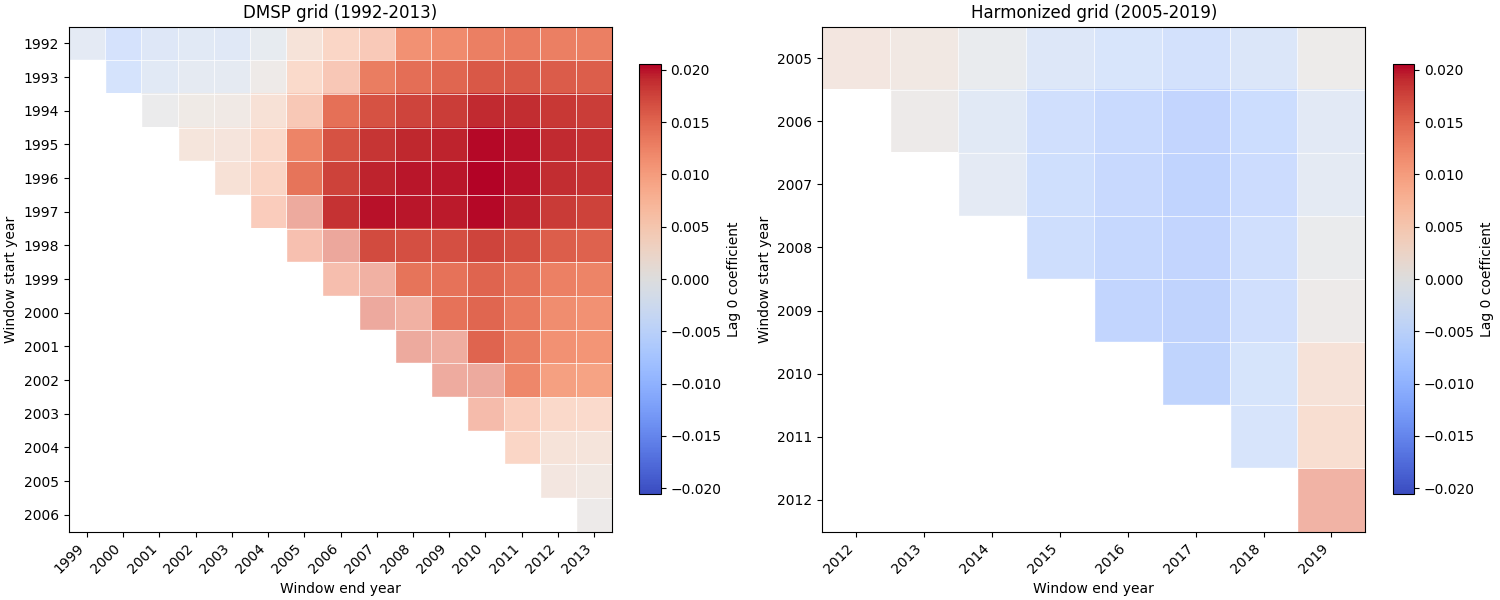
\includegraphics[width=\linewidth]{first_stage_window_grid.png}

        \column{0.38\textwidth}
        \small
        Each cell is a separate regression.
        \vspace{0.5em}
        \begin{itemize}
            \item Positive estimates cluster in DMSP windows ending late 2000s
            \item Post-2005 windows: near zero everywhere
        \end{itemize}
    \end{columns}
\end{frame}

% --- Result 3: subsamples ---
\begin{frame}{Result 3: no subsample rescues it}
    \begin{columns}[T]
        \column{0.58\textwidth}
        \centering
        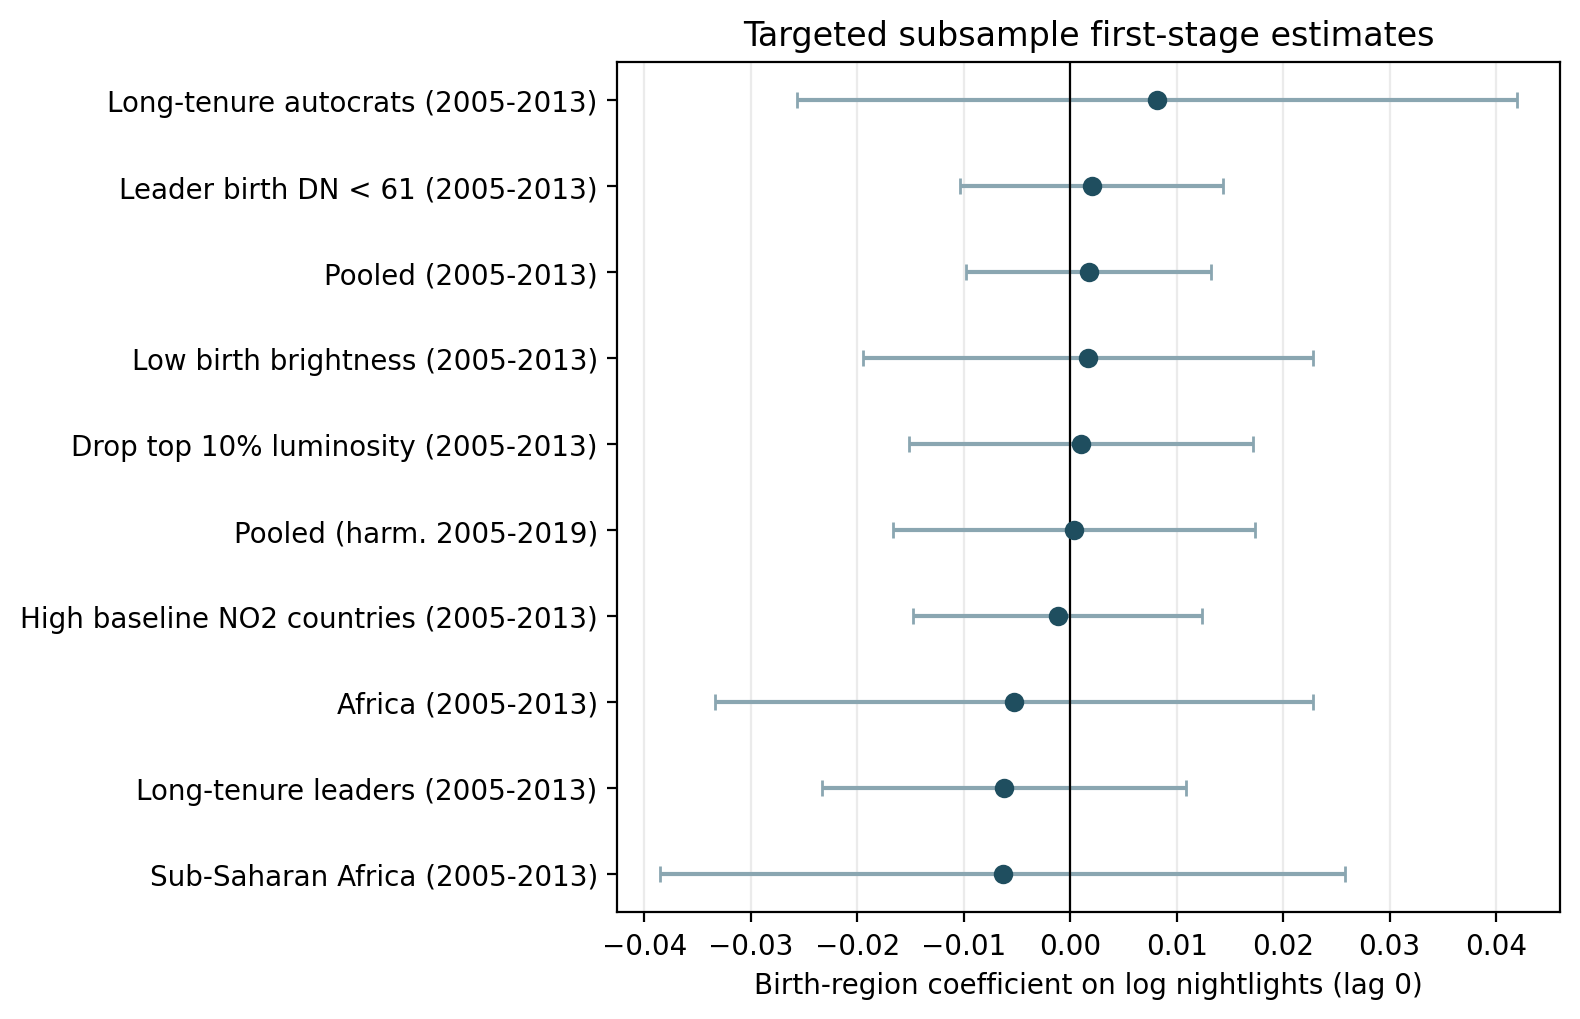
\includegraphics[width=\linewidth]{final_subsample_first_stage_plot.png}

        \column{0.42\textwidth}
        \small
        Searched where the effect should be strongest:
        \begin{itemize}
            \item Africa / SSA
            \item Long-tenure autocrats
            \item Low-brightness districts
            \item High-NO$_2$ countries
        \end{itemize}
        \vspace{0.4em}
        \textcolor{darkred}{\textbf{None passes} coef.\ $\geq 0.005$, $p < 0.10$.}
    \end{columns}
\end{frame}

% --- Result 4: pollution ---
\begin{frame}{Result 4: no green favoritism}
    \small \textcolor{darkgreen}{If favoritism shifted to cleaner growth, NO$_2$ and PM$_{2.5}$ should \emph{fall} in birth regions.}

    \vspace{0.6em}
    \centering
    \small
    \begin{tabular}{lcccc}
        \toprule
        Outcome (2005--2019, lag 0) & Coef. & SE & $p$ & N \\
        \midrule
        $\log$ Nightlights & $-0.003$ & 0.009 & 0.778 & 631k \\
        $\log$ NO$_2$ & \textcolor{darkred}{$+0.031$} & 0.015 & 0.045 & 631k \\
        NO$_2$ intensity & \textcolor{darkred}{$+0.033$} & 0.018 & 0.063 & 631k \\
        PM$_{2.5}$ intensity (lag 2) & \textcolor{darkred}{$+0.018$} & 0.007 & 0.019 & 669k \\
        \bottomrule
    \end{tabular}

    \vspace{0.8em}
    \small Estimates go the \textbf{wrong way}. Less precise under country clustering, but never negative.
\end{frame}

% --- Mechanisms ---
\begin{frame}{What could drive the attenuation?}
    \begin{itemize}
        \item Spells in the later window are shorter (5.2 $\to$ 4.0 yrs); partly mechanical
        \item Birth districts are already brighter, closer to DMSP saturation. But dropping bright districts doesn't help.
        \item Not harmonization: VIIRS-only 2018--2023 is also $\approx 0$
        \item Not worse PLAD geocoding: quality is stable across periods
        \item Green favoritism would predict falling pollution. We don't see that.
    \end{itemize}

    \vspace{0.5em}
    \begin{block}{Bottom line}
        The signal is gone, and the easy explanations don't hold.
    \end{block}
\end{frame}

% --- Takeaways ---
\begin{frame}{Takeaways}
    \begin{enumerate}
        \item The long DMSP result \textbf{still replicates}
        \item After 2005 the effect collapses --- even where theory says it should be strongest
        \item Pollution outcomes are zero-to-positive, so it isn't green favoritism
        \item A textbook political-economy result looks much weaker once you push it past 2005
    \end{enumerate}

    \vspace{1.2em}
    \begin{center}
        \Large Thank you! \\[0.4em]
        \footnotesize \texttt{github.com/RichSchulz/political-leader-pollution}
    \end{center}
\end{frame}

% ============================================
% APPENDIX
% ============================================
\appendix

\begin{frame}[noframenumbering]{Appendix: subsample activity estimates}
    \centering
    \tiny
    \begin{tabular}{llrrr}
        \toprule
        Sample & Window & Coef. & SE & $p$ \\
        \midrule
        Africa & DMSP 1992--2013 & 0.0428 & 0.0163 & 0.009 \\
        Sub-Saharan Africa & DMSP 1992--2013 & 0.0442 & 0.0174 & 0.011 \\
        Non-SSA & DMSP 1992--2013 & 0.0053 & 0.0059 & 0.370 \\
        \midrule
        Africa & DMSP 2005--2013 & $-0.0052$ & 0.0143 & 0.714 \\
        Sub-Saharan Africa & DMSP 2005--2013 & $-0.0063$ & 0.0164 & 0.700 \\
        Long-tenure leaders & DMSP 2005--2013 & $-0.0062$ & 0.0087 & 0.479 \\
        Long-tenure autocrats & DMSP 2005--2013 & 0.0081 & 0.0173 & 0.637 \\
        Drop top 10\% luminosity & DMSP 2005--2013 & 0.0010 & 0.0082 & 0.899 \\
        Low birth brightness & DMSP 2005--2013 & 0.0016 & 0.0108 & 0.880 \\
        \midrule
        Africa & Harmonized 2005--2019 & 0.0262 & 0.0189 & 0.167 \\
        Sub-Saharan Africa & Harmonized 2005--2019 & 0.0315 & 0.0210 & 0.135 \\
        \bottomrule
    \end{tabular}
\end{frame}

\end{document}
